\documentclass{article}
\usepackage{xeCJK}
\usepackage{amsmath}
\usepackage{amssymb}
\usepackage{mathrsfs}
\usepackage{xcolor}
\usepackage{bm}
\usepackage{hyperref}
\usepackage{graphicx}
\usepackage{subcaption}
\usepackage{float}
\usepackage{multicol}
\usepackage{pdfpages}
\usepackage{csquotes}
\usepackage[ruled,linesnumbered]{algorithm2e}
\usepackage[numbers, sort&compress]{natbib}

\bibliographystyle{plain}
\setlength{\parindent}{2em}
\usepackage{geometry}
\geometry{a4paper, left=2.54cm, right=2.54cm, top=3.18cm, bottom=3.18cm}

% set line spacing
% \renewcommand{\baselinestretch}{1.5}

% define reference format
\hypersetup{
    colorlinks=true,
    linkcolor=blue,
    urlcolor=blue,
    citecolor=blue,
    linkbordercolor=white
}

\title{\textbf{Phase Frustration-Induced Spatial Lattice Symmetry in the Vicsek-Kuramoto-Sakaguchi Model}}
\author{Yichen Lu}

\begin{document}

\maketitle

\tableofcontents

% \newpage
\section{The Model}

Particles have a spatial position $\mathbf{r}_i=\left( x_i, y_i \right)$ and an internal phase $\theta_i$ which evolve according to equations:
\begin{subequations} 
    \label{eq:totalDynamicsMeanField}
    \begin{align}
        \dot{\mathbf{r}}_i&=v\mathbf{p}\left( \theta _i \right)\;\label{eq:dotR},
        \\
        \dot{\theta}_i&=\frac{K}{\left| A_i \right|}\sum_{j\in A_i}{\left[ \sin \left( \theta _j-\theta _i+\alpha \right) -\sin \alpha \right]}\;\label{eq:dotTheta},
    \end{align}
\end{subequations}
for $i=1,2,\ldots,N$. Here in Eq.~(\ref{eq:dotR}), $\mathbf{p}\left( \theta \right) =\left( \cos \theta ,\sin \theta \right)$, which means each particle rotates with a constant speed $v$ in the direction of its instantaneous phase $\theta_i (t)$. 
The particles are treated as point-like with no direct spatial interactions, consistent with classical models of chiral self-propelled particles \cite{PhysRevResearch.1.023026,PhysRevLett.119.058002,Fruchart2021,PhysRevLett.127.238001,PhysRevLett.133.258302}.
As per Eq.~(\ref{eq:dotTheta}), the mean runs over neighbors within a coupling radius $d_0$ around particle $i$:
\begin{equation}
    A_i\left( t \right) =\left\{ j\mid \left| \mathbf{r}_i\left( t \right) -\mathbf{r}_j\left( t \right) \right|\leqslant d_0 \right\} \;,
\end{equation}
$K \left(\geqslant 0\right)$ is the coupling strength, $\alpha$ is the phase frustration between two neighboring particles. When $\alpha_0=0$, the dynamics reduces to the normal Vicsek-like model.
% The counter term $-\sin\alpha$ is introduced to ensure that frustration only interferes with the phase coupling without changing the sign of effective frequency.
The introduction of counter term $-\sin\alpha$ ensures that the interaction force cancels exactly when phase differences vanish ($\theta_j - \theta_i = 0$). This guarantees that perfect synchronization is always an equilibrium state. Without this term, synchronized oscillators would experience a net force $K\sin\alpha$, artificially shifting their frequencies \cite{10.1143/PTP.79.1069}.

Some necessary order parameters can be introduced to measure the level of coordination among particles in space motion and phase dynamics. Firstly, at the macroscopic level, the system may be described by the single-partial distribution $\rho \left( \mathbf{r},\theta ,t \right) $, which satisfies the normalization condition
\begin{equation}
    \int_{L\times L}{\mathrm{d}^2\mathbf{r}\int_0^{2\pi}{\mathrm{d}\theta \;\rho \left( \mathbf{r},\theta ,t \right)}}=1\;,
\end{equation}
where $L$ is the size of the system in two dimensions. Next, we define the coarse-grained spatial density $\varrho \left( \mathbf{r}, t \right) $ and the global polarization $p(\theta, t)$ density by integrating $\rho\left( \mathbf{r},\theta ,t \right)$ over the phase and spatial, respectively:
\begin{subequations}
    \begin{align}
        \varrho \left( \mathbf{r},t \right)& =\int_0^{2\pi}{\rho \left( \mathbf{r},\theta ,t \right) \mathrm{d}\theta}\;,\\
        p\left( \theta ,t \right) & =\int_{L\times L}{\rho \left( \mathbf{r},\theta ,t \right) \mathrm{d}\mathbf{r}}\;.
    \end{align}
\end{subequations}
In the homogeneous state, these quantities take uniform values $( \rho ,\varrho ,p ) =( \rho _0,\varrho _0,p_0 ) =( 1/\left( 2\pi L^2 \right) ,1/L^2,1/2\pi ) $.

To measure deviations from uniformity, we define the following single-particle order parameters:
\begin{equation}
    \rho _{\mathrm{std}}(t)=\frac{1}{1-\rho _0}\left[ \max_{\mathbf{r}\in L\times L,\ \theta \in \left[ 0,2\pi \right]} \rho \left( \mathbf{r},\theta ,t \right) -\rho _0 \right]  \;,
\end{equation}
Similarly, we can define order parameters for spatial and phase polarization densities, denoted as $\varrho _{\mathrm{std}}$ and $p_{\mathrm{std}}$, respectively.
These order parameters range from 0 to 1, reflecting the degree of spatial and phase coherence in the system. When particles are uniformly distributed in both space and phase, $\rho ,\varrho ,p_{\mathrm{std}} \approx 0$. Conversely, if full condensation and polarization occur, $\rho ,\varrho ,p_{\mathrm{std}}\approx 1$.

We conducted numerical simulations to investigate the performance and characteristics of our system under various conditions.
For simplicity, we assume that particles are initially distributed uniformly in a two-dimensional $L\times L$ square with periodic boundary conditions.
Unless otherwise stated, all the numerical simulations of the model Eq.~(\ref{eq:totalDynamicsMeanField}) were run on Python using Euler integration.
For the final state and phase diagram, each data point of order parameters was collected by averaging last 500 time steps of the simulation to discard the transients.
 

% \newpage
% \section{Phase Frustration-Induced Crystallization}

% \subsection{Key properties}

% \begin{enumerate}
%     \item \textbf{\textcolor{red}{[Done]}} What does the lattice structure look like? What is the unit cell structure, and what is the spatial arrangement of the unit cells? Besides triangular, what other spatial structures exist? In which regions of frustration does it appear? (And what are the corresponding coupling conditions and natural frequency distributions?)
    
%         Lattice structure emerges when $\alpha\in\left(\pi/2, \pi\right]$
%         For $\pi/2<\alpha\ll\pi$, the lattice structure exhibits a triangular arrangement (Sometimes it is a tetragonal lattice, but in most cases it is stable in a triangular lattice), where in each cell, particles are arranged in a vortex pattern independent of natural frequency (mainly determined by initial conditions). This arrangement leads to a stable and ordered configuration, where the cells maintain a fixed distance from each other and the particles rotate in a coordinated manner in the form of cycloids, which leads to respiration-like motion of the cells.
%         While for $\alpha=\pi$ (anti-alignment coupling), the system transforms into a double-lane structure with particles in each lane propelling in opposite directions. 
%     \item \textbf{\textcolor{red}{[Done]}} What is each cell composed of?
    
%         Each cell is composed of particles with the neighboring particles at initial conditions, whose criterion is discussed in Sec.~\ref{sec:cellComposition}. 
%     \item \textbf{\textcolor{red}{[Done]}} What is the internal dynamics within a cell?
    
%         Within a cell, particles are all-to-all coupled, and they rotate in a Kuramoto-like manner.
%     \item \textbf{\textcolor{red}{[Done]}} What determines the length (periodicity)? (Interaction distance?)

%         The lattice constant (distance) is determined by the coupling strength $K$, the radius $d_0$, and the frustration $\alpha$. For $\alpha\gtrapprox0.5\pi$ The theoretical lattice constant is given by Eq.~\eqref{eq:latticeConstant}. 
% \end{enumerate}

% \newpage
% \subsubsection{Snapshots and phase diagram}

% \begin{figure}[H]
%     \centering
%     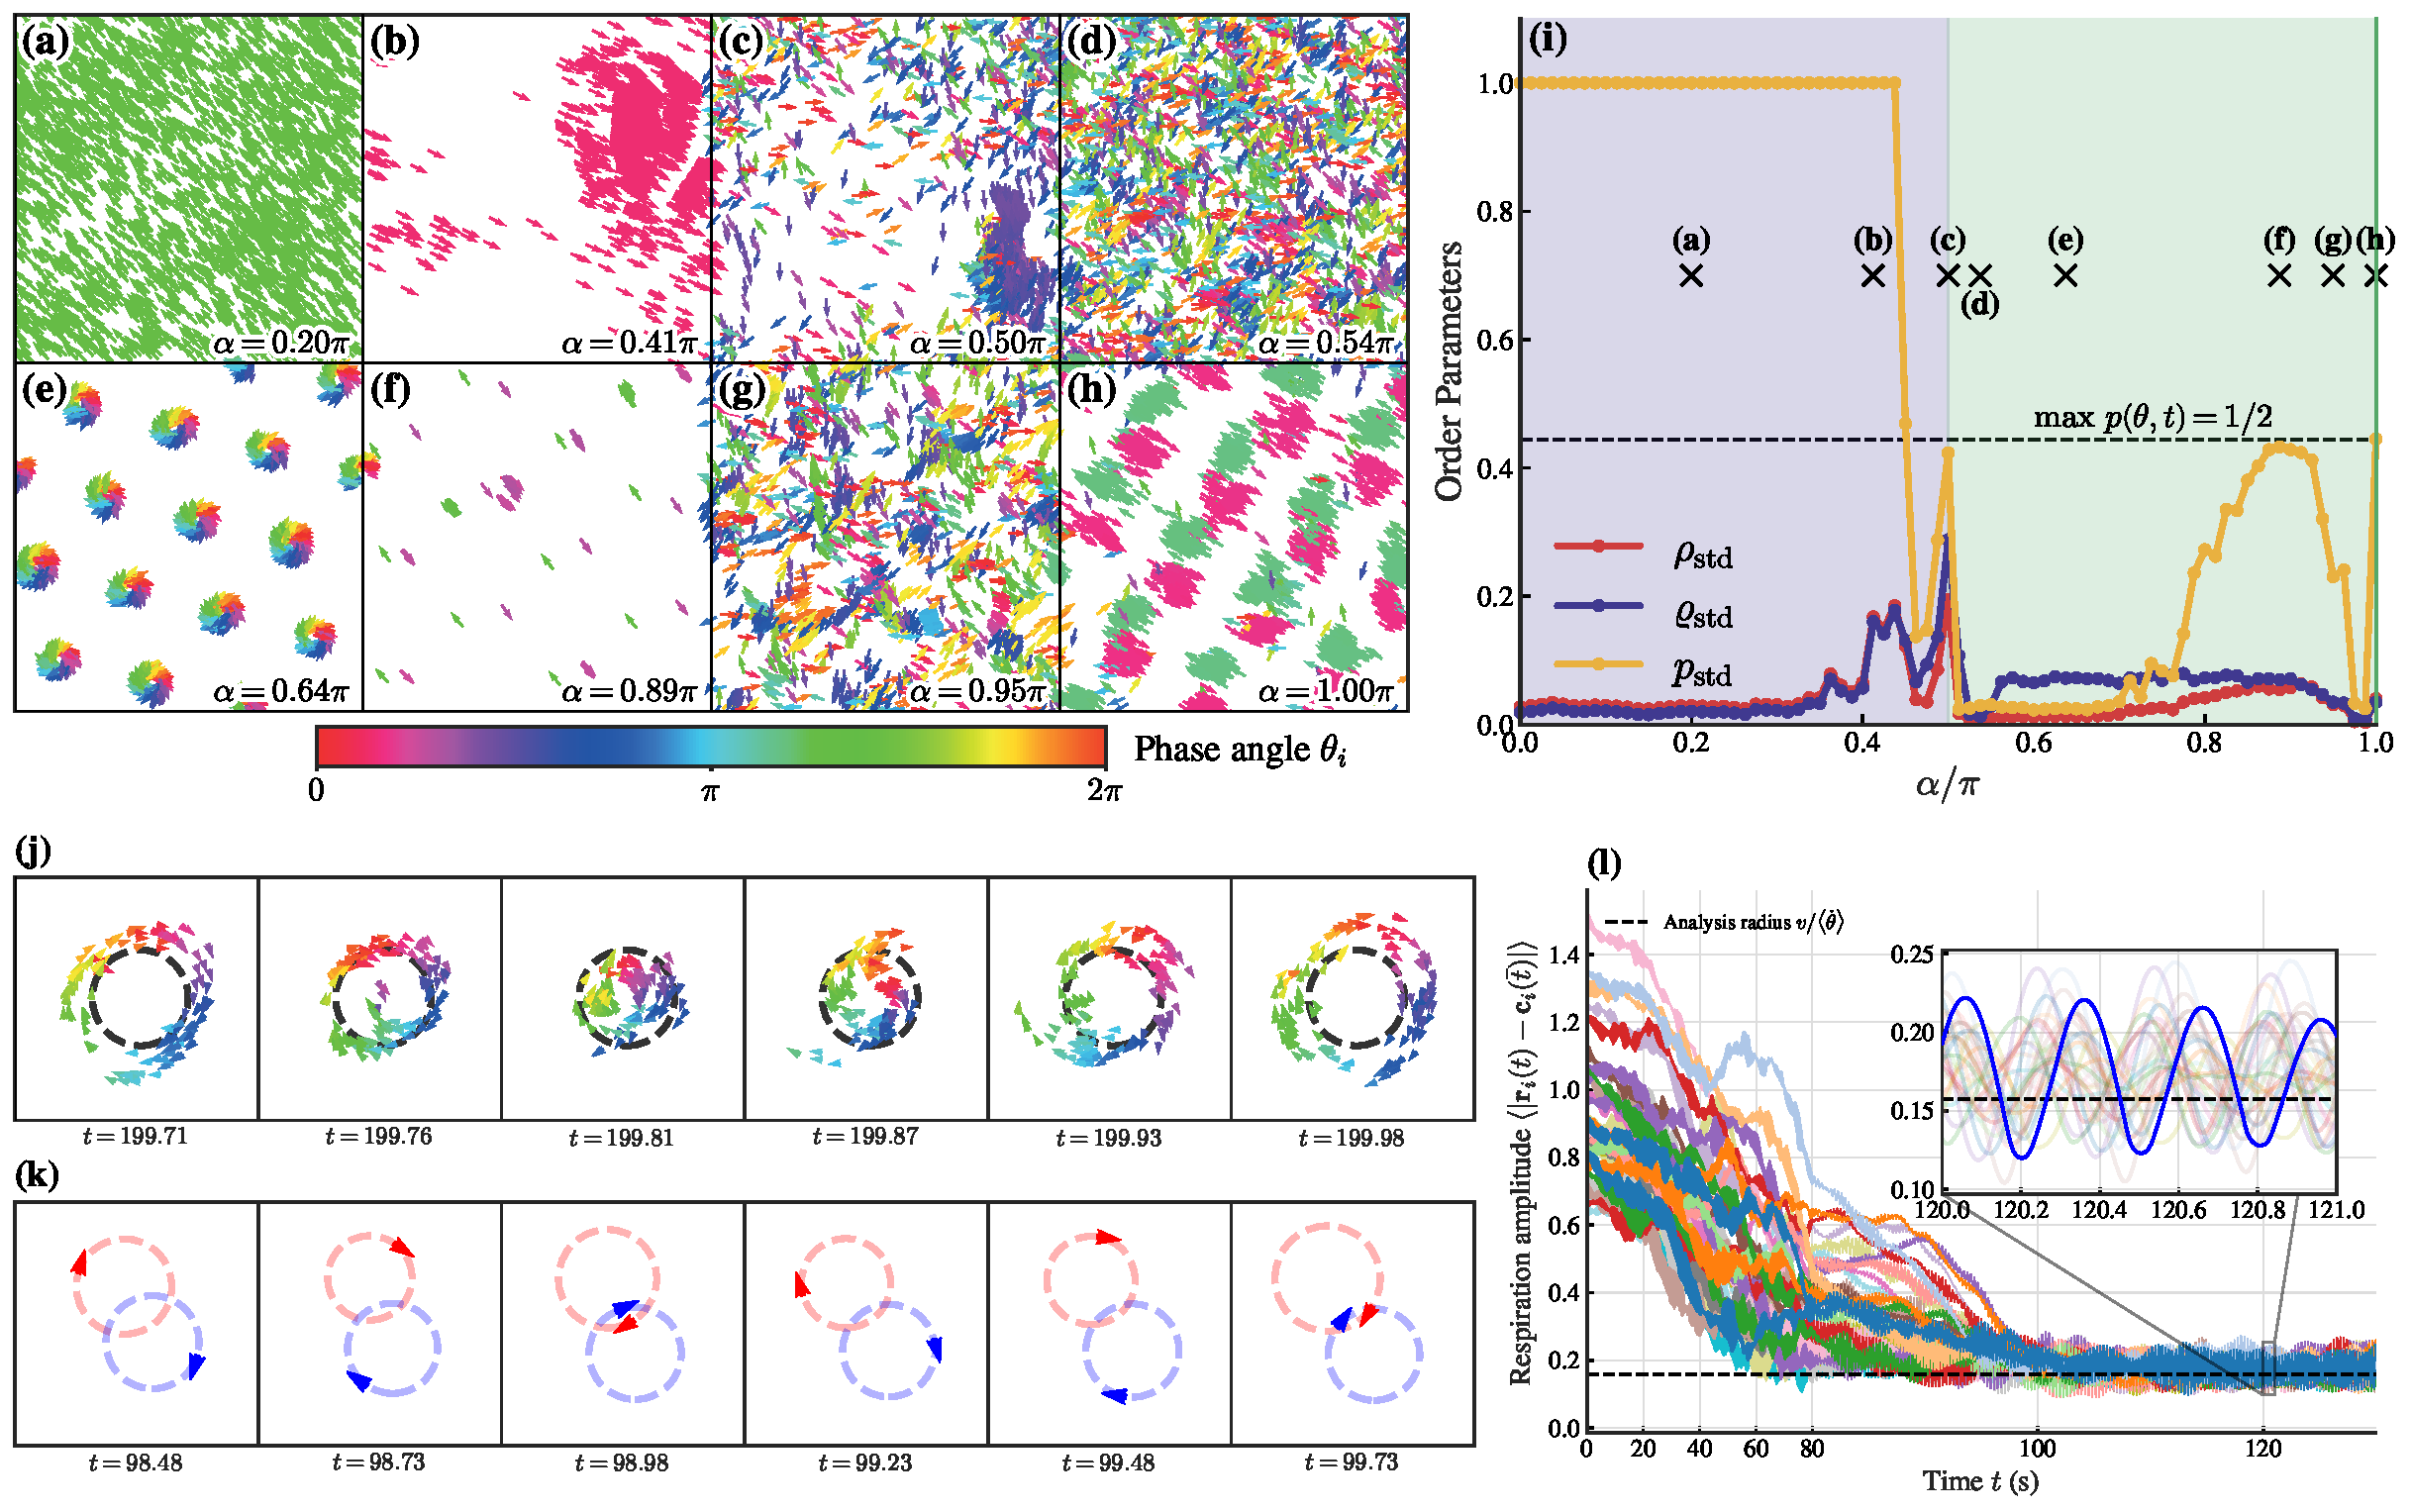
\includegraphics[width=\textwidth]{./figs/snapshotsAndPhaseDiagram.pdf}
%     \caption{
%         \label{fig:snapshotsAndPhaseDiagram}
%         (a)-(h) Representative simulation snapshots for synchronization state [(a)-(c)] and lattice state [(d)-(h)] at different phase frustration $\alpha$. The orientation and color of particles represent their instantaneous phase $\theta_i$.
%         (i) Phase diagram and order parameters of the system with respect to the phase frustration $\alpha$. The crosses mark the snapshots in (a)-(h). Regions of blue and green respectively represent the synchronization and lattice states. The horizontal dashed line indicates the values of the value of order parameter $p_{\mathrm{std}}$ when $\max p(\theta, t)=1/2$ (Dual cluster synchronization). Parameters: $K=20$, $d_0=1.55$, $L=7$.
%     }
% \end{figure}

% \begin{figure}[H]
%     \centering
%     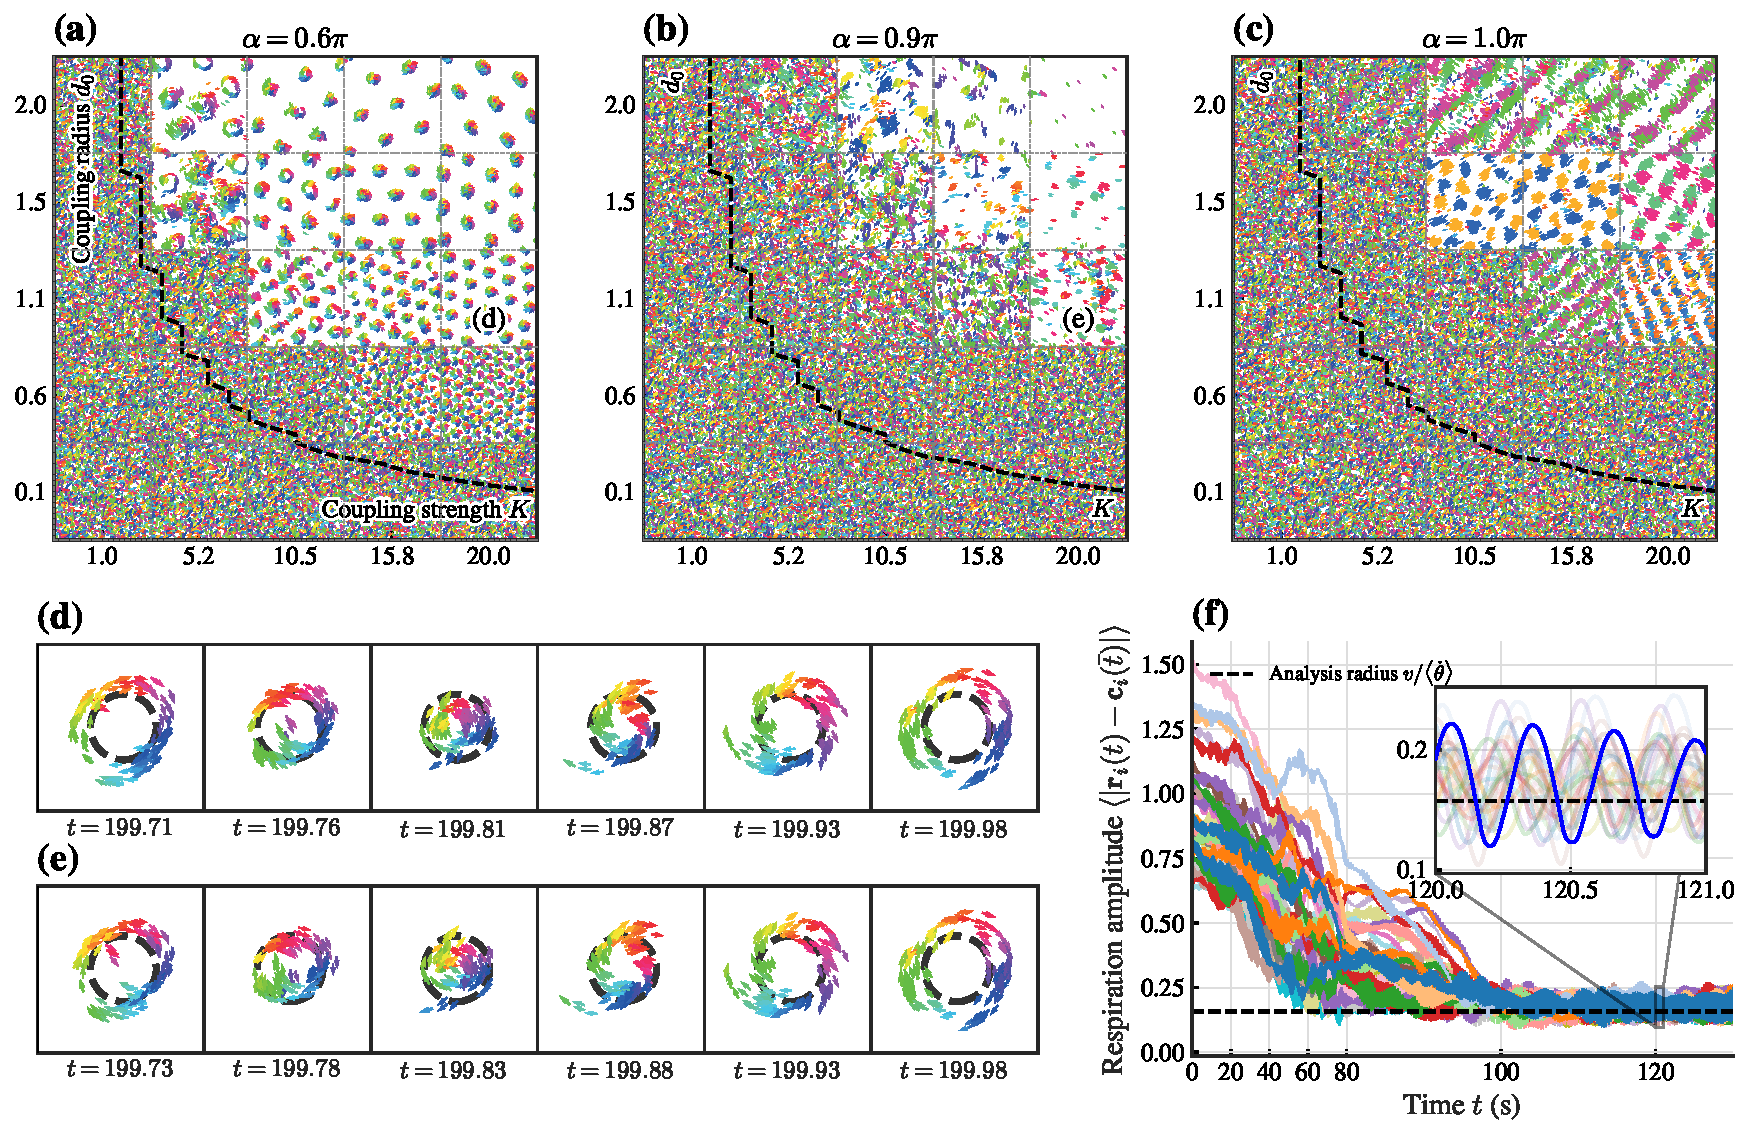
\includegraphics[width=\textwidth]{./figs/phaseDiagramAndRespiration.pdf}
%     \caption{
%         \label{fig:phaseDiagramAndRespiration}
%         (a)-(c) Snapshots of $(K, d_0)$ phase diagram for different frustration $\alpha$ at system size $L=7$. The regions of manifest and cryptic lattice states are indicated by the black dashed lines given by Eq.~\eqref{eq:criticalLineOfKD0}. (d) 
%     }
% \end{figure}

% \begin{figure}
%     \centering
%     \includegraphics[width=0.49\textwidth]{./figs/hyperuniform.pdf}
%     \caption{
%         \label{fig:hyperuniform}
%         1
%     }
% \end{figure}

\newpage

\section{\label{sec:latticeStructure}Lattice Structures and Spatiotemporal Patterns}

\begin{figure}
    \centering
    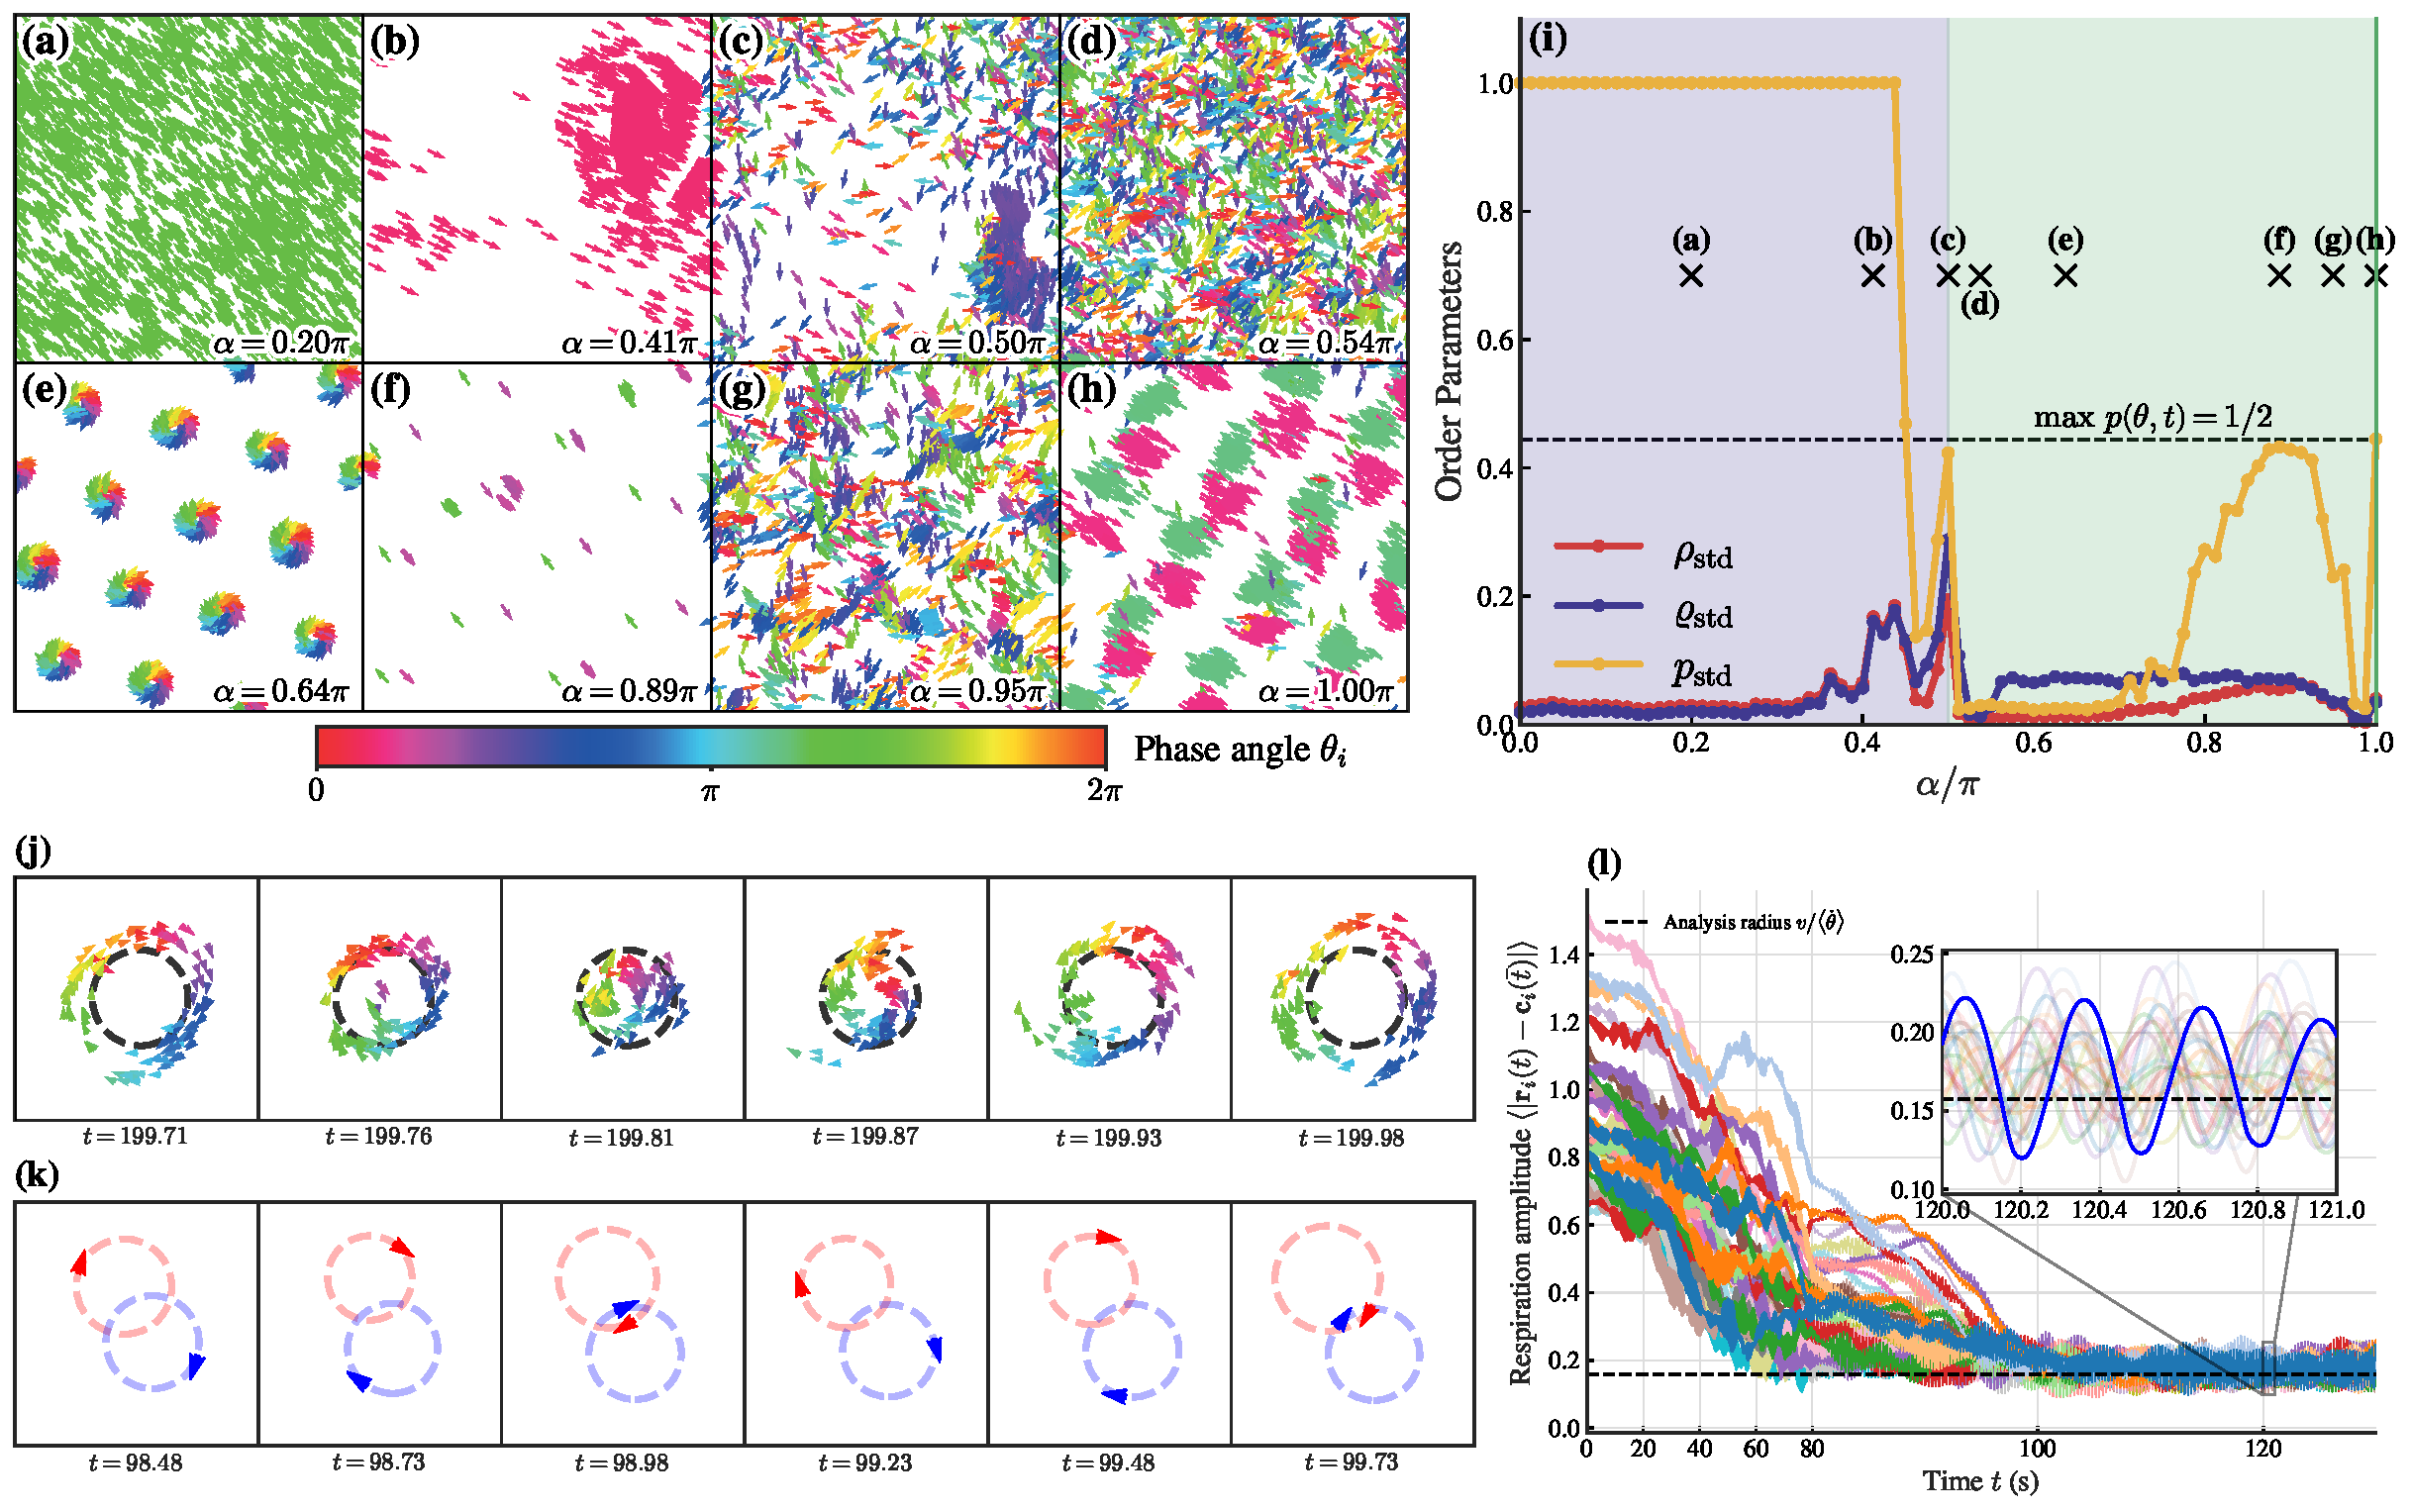
\includegraphics[width=\textwidth]{./figs/snapshotsAndPhaseDiagram.pdf}
    \caption{
        \label{fig:snapshotsAndPhaseDiagram}
        (a)-(h) Representative simulation snapshots for synchronization state [(a)-(c)] and lattice state [(d)-(h)] at different phase frustration $\alpha$. The orientation and color of particles represent their instantaneous phase $\theta_i$.
        (i) Phase diagram and order parameters of the system with respect to the phase frustration $\alpha$. The crosses mark the snapshots in (a)-(h). Regions of blue and green respectively represent the synchronization and lattice states. The horizontal dashed line indicates the values of the value of order parameter $p_{\mathrm{std}}$ when $\max p(\theta, t)=1/2$ (Dual cluster synchronization). 
        (j), (k) Time evolution of respiration motion of vortex [(j), $\alpha=0.6\pi$] and double clustered [(k), $\alpha=0.9\pi$] unit cell. 
        (k) The red and blue arrows represent the two clusters divided by their phases, and dashed circles of corresponding colors are estimated motion trajectories based on their instantaneous effective frequencies in Eq.~\eqref{eq:averageFrequency}.
        (l) Respiration amplitude revealed by the time evolution for $\alpha=0.6\pi$.
        Other parameters: $K=20$, $d_0=1.55$, $L=7, N=2000, v=3$. 
        }
\end{figure}

Our system consists of self-propelled particles with local phase interactions, leading to a rich variety of collective behaviors. As shown in Fig.~\ref{fig:snapshotsAndPhaseDiagram}(a), when the phase frustration $\alpha$ is small, the system tends to synchronize in phase, resulting in a globally synchronized state where all particles move coherently in the same direction. This state is characterized by high values of the order parameter$p_{\mathrm{std}}$ and low values of $\rho_{\mathrm{std}}$ and $\varrho_{\mathrm{std}}$, indicating uniform spatial distribution but strong phase coherence. As $\alpha$ gradually increases but still maintains continuity ($\alpha < \pi/2$), the system exhibits a swarming synchronization state, as shown in Fig.~\ref{fig:snapshotsAndPhaseDiagram}(b). In this state, particles form a large, coherent cluster that moves collectively, with phases still largely aligned. The order parameters reflect this state, with $p_{\mathrm{std}}$ remaining high, while $\rho_{\mathrm{std}}$ and $\varrho_{\mathrm{std}}$ bifurcate from zero due to the formation of the cluster. The parameter space and phenomena mentioned above have been extensively studied in previous works \cite{PhysRevE.98.032219,PhysRevE.102.022604}.
With increasing $\alpha$ beyond $\pi/2$, the system undergoes a transition to a lattice state, as shown in Fig.~\ref{fig:snapshotsAndPhaseDiagram}(d)-(h). In this state, particles arrange themselves into a hexagonal lattice structure, breaking the spatial uniformity. The order parameters reflect this change, with $\rho_{\mathrm{std}}$ and $\varrho_{\mathrm{std}}$ non-zero significantly remaining constant over a large range ($0.55\pi<\alpha<0.9\pi$), indicating the formation of spatial patterns. $p_{\mathrm{std}}$ decreases at first ($0.5\pi<\alpha<0.7\pi$, the vortex lattice state, Fig.~\ref{fig:snapshotsAndPhaseDiagram}(e)), showing reduced phase coherence, but then increases again ($0.7\pi<\alpha<\pi$), indicating the emergence of dual-cluster synchronization where particles form two distinct phase clusters (Fig.~\ref{fig:snapshotsAndPhaseDiagram}(f)). This dual-cluster state is characterized by two dominant phases that differ by $\pi$, leading to a bimodal distribution in $p(\theta, t)$. 
Continuing to increase $\alpha$ towards $\pi$, the three order parameters decrease again, indicating a return to a more disordered state (Fig.~\ref{fig:snapshotsAndPhaseDiagram}(g)).
While at $\alpha = \pi$, system reaches a state of perfect anti-synchronization, where neighboring particles have phases differing by $\pi$, leading to a dual-lane pattern in space and dual-cluster synchronization in phase (Fig.~\ref{fig:snapshotsAndPhaseDiagram}(h)). Different from the previous dual-cluster state in Fig.~\ref{fig:snapshotsAndPhaseDiagram}(f), here the two phase clusters are fixed, resulting in a continuous linear arrangement of motion in space. This pattern has also been observed in Escaff's work on anti-aligning interactions \cite{PhysRevE.109.024602,PhysRevE.110.024603}

For a more detailed understanding of the spatiotemporal pattern for lattice states, we examined the time evolution of individual unit cells in the vortex lattice and dual-cluster states, as shown in Fig.~\ref{fig:snapshotsAndPhaseDiagram}(j) and (k). In the vortex lattice state (Fig.~\ref{fig:snapshotsAndPhaseDiagram}(j)), particles within a unit cell exhibit a respiration motion, where they periodically expand and contract around their analysis average radius $v/\langle \dot{\theta} \rangle$, where $\langle \dot{\theta} \rangle$ is given by the phase dynamics in incoherent states
\begin{equation}
    \begin{aligned}
        \langle \dot{\theta}\rangle &=-K\sin \alpha +\frac{K}{2\pi}\int_0^{2\pi}{\mathrm{d}\theta ^{\prime}\sin \left( \theta ^{\prime}-\theta +\alpha \right)}\\
        &=-K\sin \alpha\;.\\
    \end{aligned}  
    \label{eq:averageFrequency}
\end{equation}
This dynamic behavior is characterized by oscillations in the distance between particles and the centers of their unit cells $\left| \mathbf{r}_i\left( t \right) -\mathbf{c}_i\left( \bar{t} \right) \right|$, as illustrated in Fig.~\ref{fig:snapshotsAndPhaseDiagram}(l), where $\mathbf{c}_i\left( \bar{t} \right)$ is the center of the unit cell averaged over one period. 
The amplitude of these oscillations provides insight into the stability of the lattice structure (see Hopf–Turing bifurcation in Sec.~\ref{sec:mechanism}). As respiration motion, compared to the vortex lattice state, the dual-cluster state (Fig.~\ref{fig:snapshotsAndPhaseDiagram}(k)) shows a more ordered arrangement, with two groups of particles rotating around the center of the unit cell in opposite directions along approximately fixed trajectory (Note that they are not only two particles but two groups of particles fully condensed). The trajectories of these two groups can be approximated by circles with radii determined by their instantaneous effective frequencies in Eq.~\ref{eq:averageFrequency}, as indicated by the dashed circles in Fig.~\ref{fig:snapshotsAndPhaseDiagram}(k). 

% \vspace{l}

% \begin{figure}[H]
%     \centering
%     \includegraphics[width=\textwidth]{./figs/snapshot_v_alpha_K16.83_d01.55.pdf}
%     \caption{
%         Snapshot of the achiral system ($\omega _{\min}=0$, $\Delta \omega=0$) at $t=200$ with $N=2000$, $K=16.83$, and $d_0=1.55$.
%     }
% \end{figure}

% \begin{figure}[H]
%     \centering
%     \includegraphics[width=\textwidth]{./figs/snapshot_v_alpha_K20.00_d01.00.pdf}
%     \caption{
%         Snapshot of the achiral system ($\omega _{\min}=0$, $\Delta \omega=0$) at $t=200$ with $N=2000$, $K=20$, and $d_0=1$.
%     }
% \end{figure}

% \newpage
% The phase diagram of the system is constructed by varying the key parameters, including the coupling strength $K$, the radius $d_0$. The resulting patterns are classified into ordered and lattice states. 

% Single chirality particles can also form a triangular lattice structure:
% \begin{figure}[H]
%     \centering
%     \includegraphics[width=0.9\textwidth]{./figs/asymmetric.png}
%     \caption{
%         Snapshots of asymmetric chiral system ($\omega _{i}\sim[0, 2]$) at different coupling strengths $K$ and radius $d_0$ for $\alpha = 0.6\pi$.
%     }
% \end{figure}
% \vspace{-0.5cm}
% \begin{figure}[H]
%     \centering
%     \includegraphics[width=0.9\textwidth]{./figs/uniform.pdf}
%     \caption{
%         The probability distribution functions (PDF) of distances, $r$, normalized with the mean particle spacing, $r_0$.
%         The dash line is the PDF of Rayleigh Distribution $P(r)=2\pi r\exp\left[-\pi r^2\right]$.
%     }
% \end{figure}

% \begin{figure}[H]
%     \centering
%     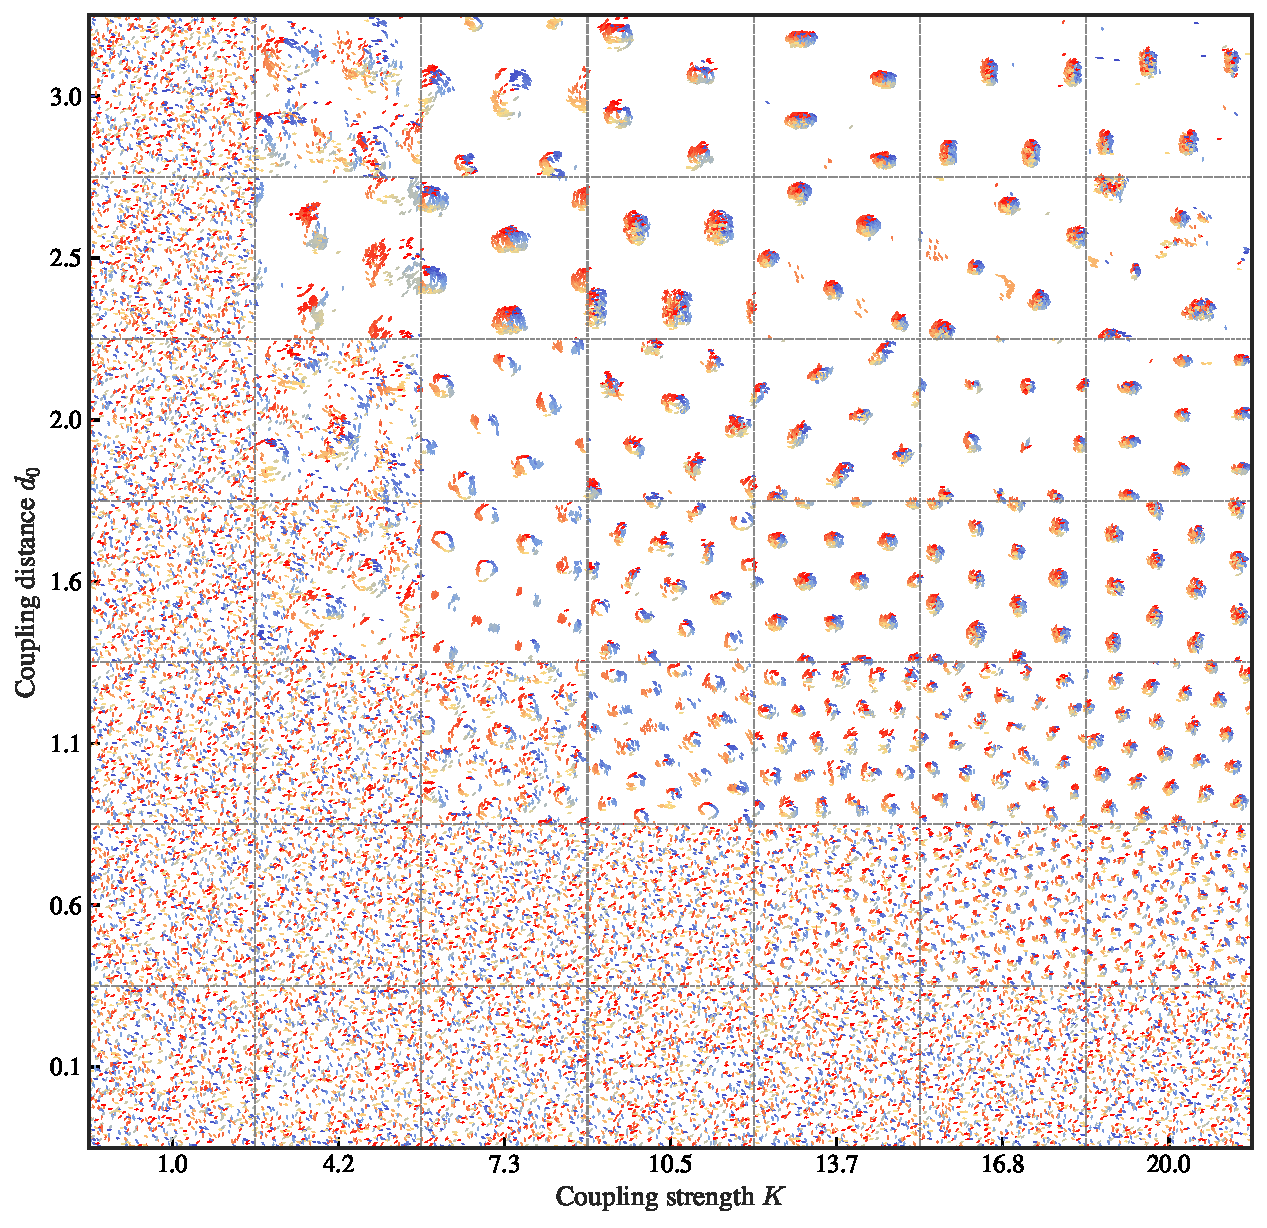
\includegraphics[width=\textwidth]{./figs/snapshot0.6pi.pdf}
%     \caption{
%         Snapshots of achiral system ($\omega _{\min}=0$ and $\Delta \omega=0$) at different coupling strengths $K$ and radius $d_0$ for $\alpha = 0.6\pi$. 
%     }
% \end{figure}

% \begin{figure}[H]
%     \centering
%     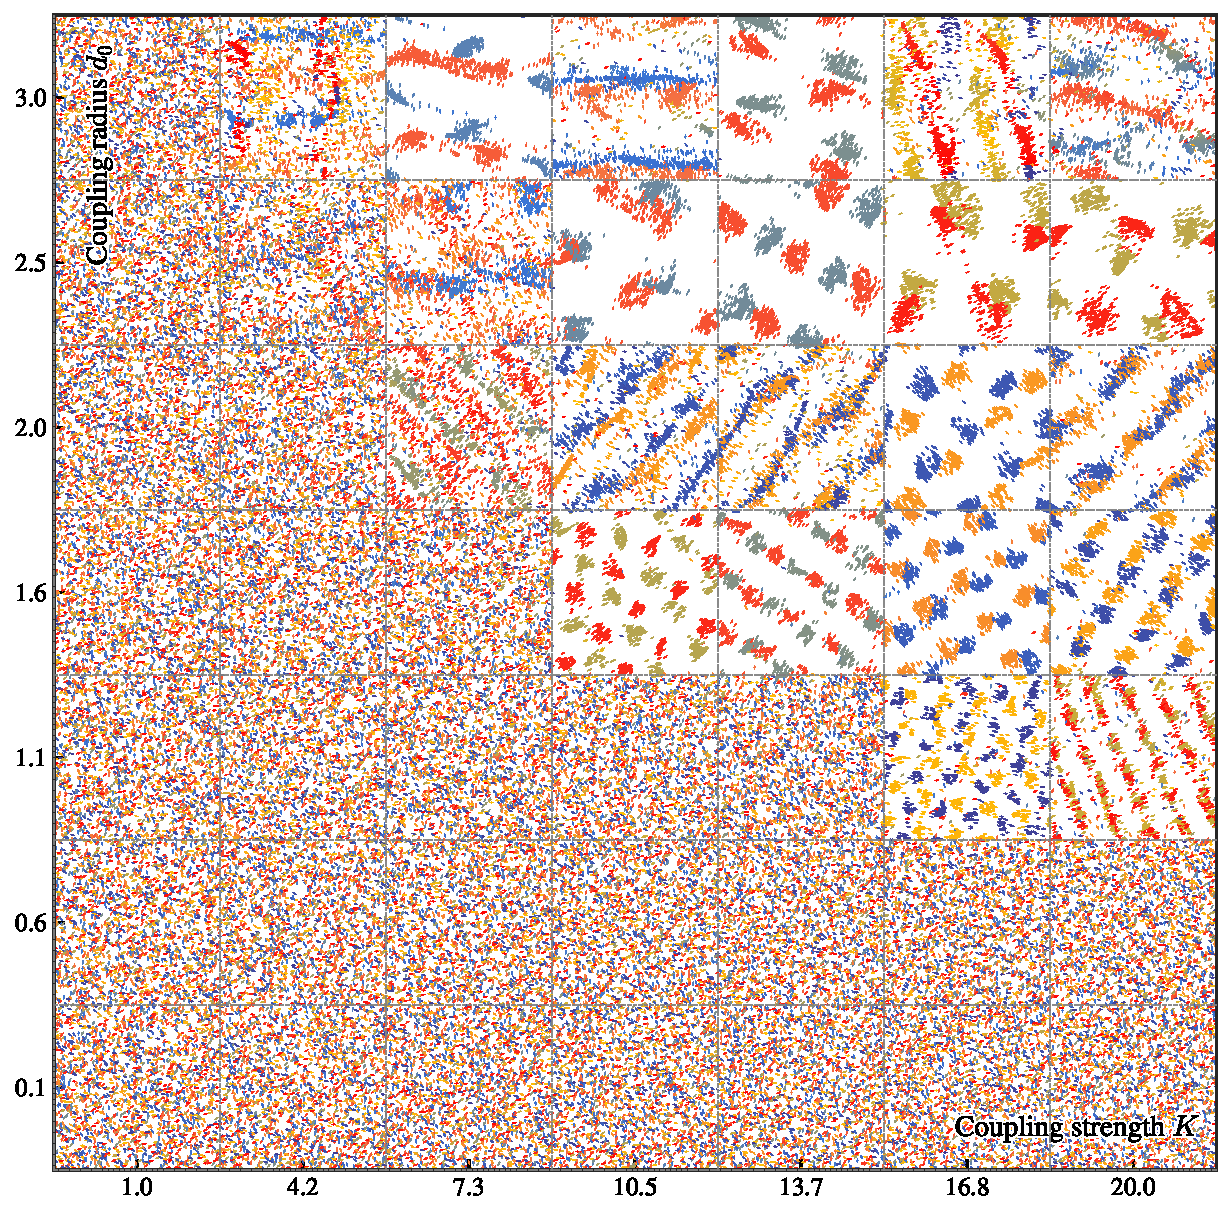
\includegraphics[width=\textwidth]{./figs/PhaseLagPatternFormation_varying_strengthK_and_distanceD0_phase_a3.14_Do0_aN2000_distuniform.pdf}
%     \caption{
%         Snapshots of achiral system ($\omega _{\min}=0$ and $\Delta \omega=0$) at different coupling strengths $K$ and radius $d_0$ for $\alpha = \pi$. 
%     }
% \end{figure}

% \begin{figure}[H]
%     \centering
%     \includegraphics[width=\textwidth]{./figs/PhaseLagPatternFormation_varying_strengthK_and_distanceD0_phase_a1.88_Do0_aN2000_distuniform.png}
%     \caption{
%         \label{fig:snapshot0.6pi_chiral}
%         Snapshots of achiral system ($\omega _{\min}=0$ and $\Delta \omega=0$) at different coupling strengths $K$ and radius $d_0$ for $\alpha = 0.6\pi$ with higher granularity. 
%     }
% \end{figure}

% \begin{figure}[H]
%     \centering
%     \includegraphics[width=0.7\textwidth]{./figs/orderParameter_varying_strengthK_and_distanceD0.png}
%     \caption{
%         \label{fig:orderParameter_varying_strengthK_and_distanceD0}
%         The order parameter $\sigma _{\rho}\left( t \right)$ as a function of coupling strength $K$ and radius $d_0$(Corresponding to Fig.~\ref{fig:snapshot0.6pi_chiral}). The color indicates the value of the order parameter.
%     }
% \end{figure}

\newpage
\subsection{Respiration-like motion of unit cells}

For $\alpha=0.6\pi$, the system exhibits the respiration-like motion of the cells. Since the phases of particles in each cell are uniformly distributed in $[0, 2\pi]$ and the distance between cells is large enough to be considered decoupled, the effective frequency of each particle can be approximated by
\begin{equation}
    \dot{\theta}_i=-K\sin \alpha +\frac{K}{\left| A_i \right|}\int_0^{2\pi}{\mathrm{d}\theta ^{\prime}\sin \left( \theta ^{\prime}-\theta _i+\alpha \right)}=-K\sin \alpha\;,
\end{equation}
and the lattice constant $a$ can be approximated as 
\begin{equation}
    a=d_0+2\frac{v}{K\left| \sin \alpha \right|}\;.
    \label{eq:latticeConstant}
\end{equation}
\begin{figure}[H]
    \centering
    \includegraphics[width=\textwidth]{./figs/respiration_snapshot.pdf}
    \caption{
        \label{fig:respiration_snapshot}
        respiration-like motion of the cells with $\omega _{\min}=0$, $\Delta \omega=0$, $N=3000$, $K=10.5$, $d_0=1.07$, and $\alpha=0.6\pi$. Black hollow dots represent the center of mass of each cell, black dash circles represent the theoretical unit cell radius $v/\dot{\theta}_i$, and the gray dash lines represent the theoretical distance between unit cells $d_0$.
    }
\end{figure}
\begin{figure}[H]
    \centering
    \includegraphics[width=0.5\textwidth]{./figs/respiration_amplitude_inset.pdf}
    \caption{
        \label{fig:respiration_amplitude}
        respiration amplitude of the system. 
        The parameters are the same as in Fig.~\ref{fig:respiration_snapshot}.
        Different colors represent different cells, and the amplitude is defined as the distance between particles and the center of mass of the cell at final state ($\bar{t}=40$).
    }
\end{figure}
As shown in Fig.~\ref{fig:respiration_snapshot} and Fig.~\ref{fig:respiration_amplitude}, the respiration amplitude of the cells is defined as $\left< \left| \mathbf{r}_i\left( t \right) -\mathbf{c}_i\left( \bar{t} \right) \right| \right> $, where $\mathbf{c}_i(\bar{t})$ is the center of mass of the cell of $i$-th particle at final state ($\bar{t}=40$), and $\left< \cdot \right>$ denotes the average over all particles in the cell. It is worth noting that the amplitude is fluctuating around the theoretical cell radius $v/\dot{\theta}_i$ and the
respiration frequency of the cells exhibit synchronization.

\begin{figure}[H]
    \centering
    \includegraphics[width=\textwidth]{./figs/respiration_snapshot_decoupled.pdf}
    \caption{
        respiration-like motion of the decoupled cells. The parameters are the same as in Fig.~\ref{fig:respiration_snapshot}.
    }
\end{figure}

\begin{figure}[H]
    \centering
    \includegraphics[width=0.5\textwidth]{./figs/respiration_amplitude_cells_decouled.pdf}
    \caption{
        Respiration amplitude of the decoupled cells ($t > 80$). The parameters are the same as in Fig.~\ref{fig:respiration_snapshot}.
    }
\end{figure}

\newpage
\section{\label{sec:hyperuniformity}Dominant-Recessive Lattice and Hyperuniformity}

\begin{figure}
    \centering
    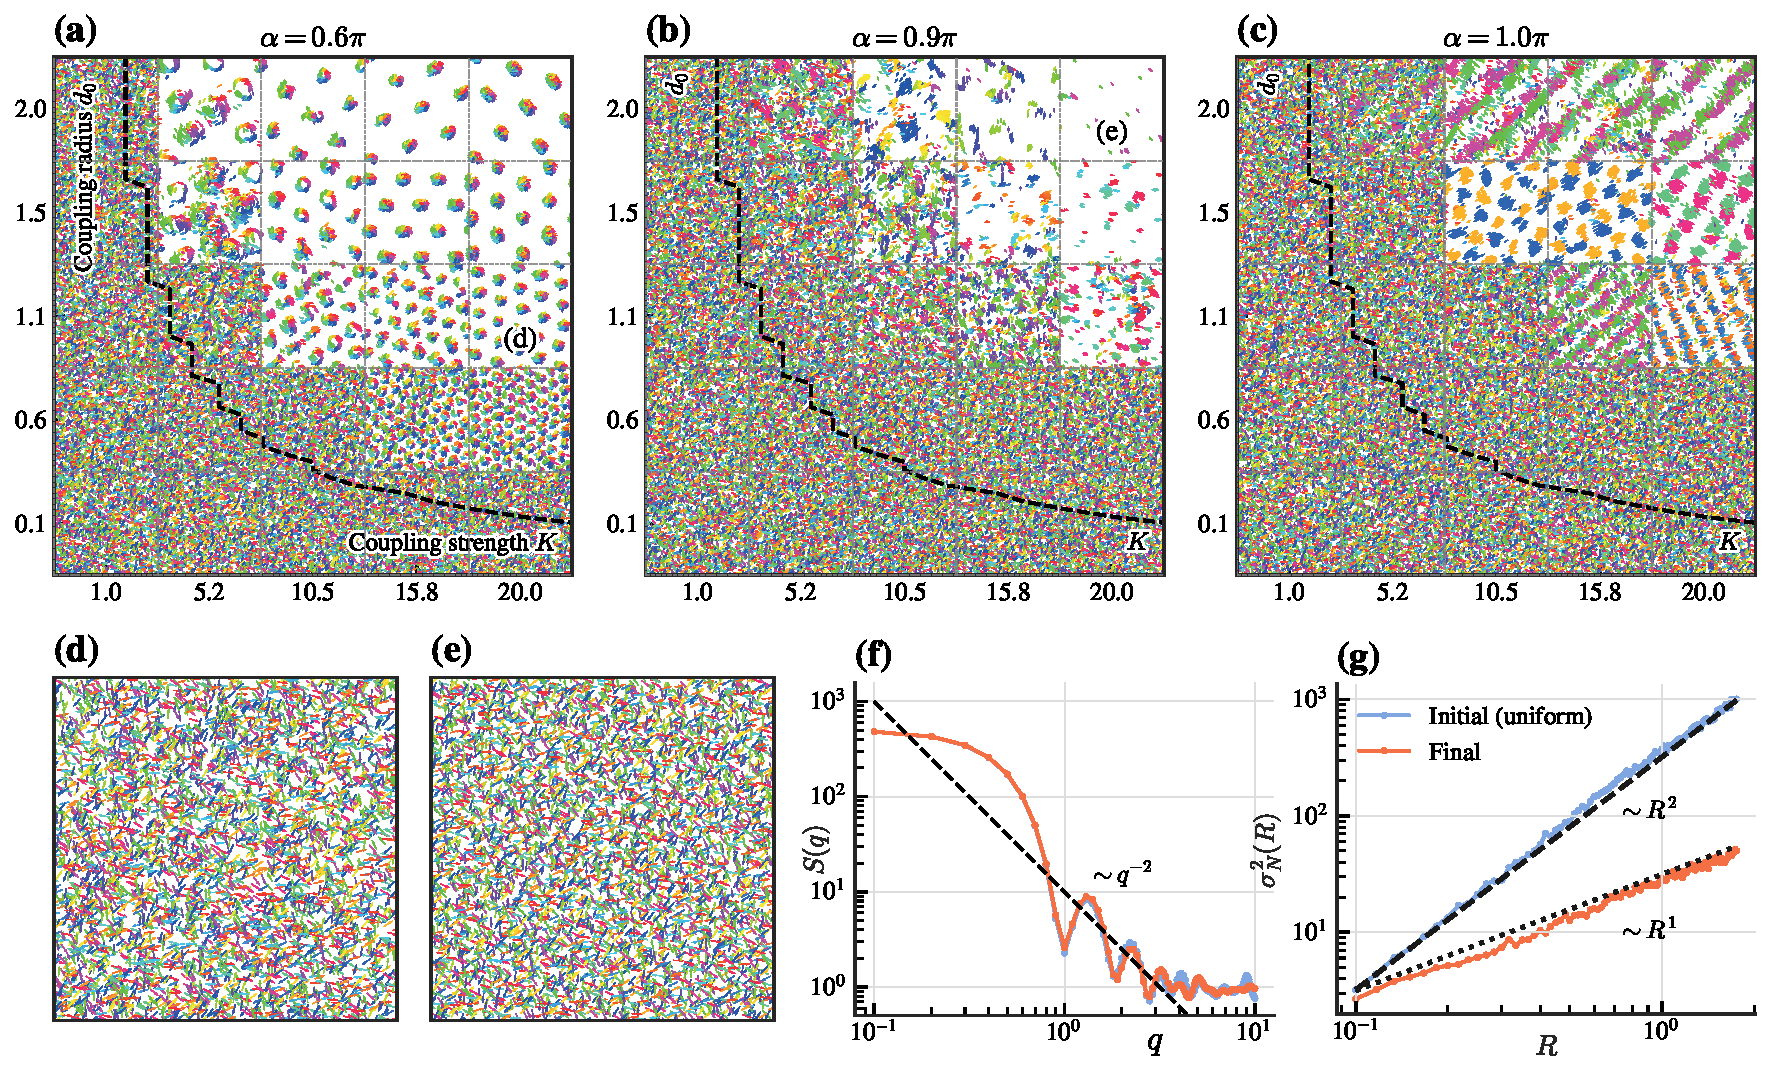
\includegraphics[width=\textwidth]{./figs/phaseDiagramAndHyperuniformity.pdf}
    \caption{
        \label{fig:phaseDiagramAndHyperuniformity}
        (a)-(c) Snapshots of $(K, d_0)$ phase diagram for different frustration $\alpha$ at population $N=2000$. The regions of dominant and recessive lattice states are indicated by the black dashed lines given by Eq.~\eqref{eq:criticalLineOfKD0}. Other parameters: $L=7, v=3$.
        (d), (e) Snapshots of random uniform (d, initial conditions) and hyperuniform (e, final state of (d)) for $K=20, d_0=0.25, N=5000, \alpha=0.6\pi$.
        Hyperuniformity of (d) and (e) is characterized by the structure factor $S(q)$ (f) and number variance $\sigma _N^2(R)$ (g). The black dashed lines indicate the scaling behaviors $S(q)\sim q^{-2}$ and $\sigma _N^2(R)\sim R^{1,2}$, respectively.
    }
\end{figure}

As discussed above, the lattice state emerges when the phase frustration $\alpha$ exceeds a critical value of $\pi/2$, and $\alpha$ mainly controls the topology of the lattice pattern.
However, the prominence of this lattice structure depends on the coupling strength $K$ and coupling radius $d_0$.
As shown in Fig.~\ref{fig:phaseDiagramAndHyperuniformity}(a)-(c), for a given $\alpha$, there exists a region in the top right of $(K, d_0)$ parameter space where the lattice structure is dominant, characterized by long lattice constants (the average distance between neighboring unit cells) and high volume fractions (the area occupied by particles within a unit cell) of unit cells.
Within this region, the lattice constant increases with $d_0$ but is insensitive to $K$. Conversely, the volume of the unit cell decreases with increasing $K$ but is insensitive to $d_0$.
Outside this region, the lattice structure becomes recessive, and the system tends to return to a more uniform state. The boundary between these regions can be approximated by the relation \eqref{eq:criticalLineOfKD0} (see Sec.~\ref{sec:mechanism} for details), which balances the spatial periodicity of pattern formation and the spatial dynamics of particles.

Interestingly, even in the recessive lattice region, where the system appears macroscopically uniform, it still exhibits microscopic hyperuniformity, as shown in Fig.~\ref{fig:phaseDiagramAndHyperuniformity}(e).
To quantify the degree of order in hyperuniformity, we computed the structure factor $S(q)=N^{-1}\sum_{i,j=1}^{N}e^{i\mathbf{q}\cdot(\mathbf{r}_i-\mathbf{r}_j)}$ and number variance $\sigma _N^2(R)=\langle \left[ N\left( R \right) -\langle N\left( R \right) \rangle \right] ^2\rangle $, which are standard measures for characterizing hyperuniformity\cite{TORQUATO20181}. 

% \newpage
% \subsubsection{Lattice constant}

% \begin{figure}[H]
%     \centering
%     \subcaptionbox{
%         Continuous spectrum $\mathrm{Re}[ \lambda _{m}^{\left[ 0 \right]}\left( k \right) ]$ as a function of wave number $k$ for $K=20, d_0=1$.
%     }[0.49\linewidth]{
%         \includegraphics[width=\linewidth]{./figs/continuous_spectrum.pdf}
%     }
%     \hfill
%     \subcaptionbox{
%         Mean lattice constant $a$ versus the most unstable wave number $k^*$ (defined as the maximum point of $\mathrm{Re}[ \lambda _{m}^{\left[ 0 \right]}\left( k \right) ]$).
%     }[0.49\linewidth]{
%         \includegraphics[width=\linewidth]{./figs/lattice_constant_vs_kstar_discrete.pdf}
%     }
%     \caption{
%         Lattice constant $a$ as a function of coupling strength $K$ and radius $d_0$ for $\alpha=0.6\pi$.
%     }
% \end{figure}

% \begin{figure}[H]
%     \centering
%     \subcaptionbox{
%         1111
%     }[0.49\linewidth]{
%         \includegraphics[width=\linewidth]{./figs/initDistribution.png}
%     }
%     \hfill
%     \subcaptionbox{
%         2222
%     }[0.49\linewidth]{
%         \includegraphics[width=\linewidth]{./figs/finalDistribution.png}
%     }
%     \caption{
%         The probability distribution functions (PDF) of distances, $r$, normalized with the mean particle spacing, $r_0$.
%         The dash line is the PDF of Rayleigh Distribution $P(r)=2\pi r\exp\left[-\pi r^2\right]$.
%     }
% \end{figure}

% \newpage
% \subsubsection{Initial conditions determined cells composition \label{sec:cellComposition}}

% \begin{figure}[H]
%     \centering
%     \subcaptionbox{Initial conditions of half on each side.}[0.49\linewidth]{
%       \includegraphics[width=\linewidth]{figs/halfSide.png}
%     }
%     \hfill
%     \subcaptionbox{
%         Initial conditions of chessboard pattern.
%     }[0.49\linewidth]{
%       \includegraphics[width=\linewidth]{figs/chess.png}
%     }
%     \caption{
%         Two artificial non-uniform initial conditions in space. Red and blue particles represent particles with positive and negative chirality, respectively. 
%     }
% \end{figure}

% \begin{figure}[H]
%     \centering
%     \includegraphics[width=\textwidth]{./figs/HalfInitPhaseLagPatternFormation_a0.00_Do1_aN1000_distuniform.pdf}
%     \caption{
%         \label{fig:half}
%         Snapshot of the system at $t=80$ with $N=1000$, $K=20$, $\omega _{\min}=0$, $\Delta \omega=1$ and initial conditions of half on each side.
%     }
% \end{figure}

% \begin{figure}[H]
%     \centering
%     \includegraphics[width=\textwidth]{./figs/ChessboardPhaseLagPatternFormation_a0.00_Do1_aN1000_distuniform.pdf}
%     \caption{
%         \label{fig:chess}
%         Snapshot of the system at $t=80$ with $N=1000$, $K=20$, $\omega _{\min}=0$, $\Delta \omega=1$ and initial conditions of chessboard pattern.
%     }
% \end{figure}

% \newpage

% \begin{figure}[H]
%     \centering
%     \includegraphics[width=0.75\textwidth]{./figs/PhaseLagPatternFormation_varying_strengthK_and_distanceD0_freq_a1.88_Do1_aN1000.pdf}
%     \caption{
%         \label{fig:snapshot0.6pi_chiral}
%         Snapshots of system at different coupling strengths $K$ and radius $d_0$ with $N=1000$, $K=20$, $\alpha =0.6\pi$, $\omega _{\min}=0$, and $\Delta \omega =1$. 固定阻锉为$0.6\pi$,不同的耦合强度$K$和半径$d_0$下的手性粒子系统快照。粒子颜色根据其瞬时相位$\theta_i$着色。随着两个耦合参数的增加,粒子在空间中逐渐形成三角晶格结构且尺寸和彼此距离不断增加。
%     }
% \end{figure}

% \begin{figure}[H]
%     \centering
%     \includegraphics[width=\textwidth]{./figs/noncounter_snapshot.pdf}
%     \caption{
%         Snapshot of the system without counter term $-\sin\alpha$ at $t=80$ with $N=1000$, $K=20$, $\omega _{\min}=0.1$ and $\Delta \omega=1$. The particles are colored according to their instantaneous phase $\theta_i$. There is no triangular lattice structure, and the particles are randomly distributed in space.
%         系统终态的快照,粒子颜色根据其瞬时相位$\theta_i$着色。空间排列没有三角晶格结构,粒子在空间中随机分布。
%     }
%     \label{fig:noncounter_shotsnaps}
% \end{figure}

% \begin{figure}[H]  % 如果希望把图片放在当前段落中,可以使用[H]选项
%     \centering
%     \subcaptionbox{Snapshot}[0.49\linewidth]{
%       \includegraphics[width=\linewidth]{figs/snapshot.pdf}
%     }
%     \hfill
%     \subcaptionbox{
%         Statistics of cells
%     }[0.49\linewidth]{
%       \includegraphics[width=\linewidth]{figs/statistics.pdf}
%     }
%     \caption{
%         Snapshot and statistics of cells of system at $t=80$ with $N=1000$, $K=20$, $\alpha =0.6\pi$, $\omega _{\min}=0.1$, and $\Delta \omega =1$. In \textbf{(b)}, the pie chart shows the proportion of two chiralities in the cell, and the black, white text indicates the mean natural frequency of positive, negative chiral particles in the cell, respectively.
%         系统终态的快照和晶格统计。快照中,粒子晶格呈现三角形晶格结构。饼图显示了正负两种粒子在晶格中的比例,黑色和白色文本分别表示正负粒子的平均自然频率。
%     }
% \end{figure}

% 陆羿辰:从统计结果中看不出临近晶格之间的规律,似乎和粒子数目以及粒子的自然频率无关。

% \begin{figure}[H]  % 如果希望把图片放在当前段落中,可以使用[H]选项
%     \centering
%     \subcaptionbox{
%         Colors represent the mean natural frequency
%     }[0.49\linewidth]{
%       \includegraphics[width=\linewidth]{figs/mean_freq.pdf}
%     }
%     \hfill
%     \subcaptionbox{
%         Colors represent the mean effective frequency
%     }[0.49\linewidth]{
%       \includegraphics[width=\linewidth]{figs/mean_eff_freq.pdf}
%     }
%     \caption{
%         \label{fig:mean_freq}
%         The mean natural frequency and effective frequency of particles in each cell. The effective frequency is defined as the average instantaneous phase velocity of particles in the cell.
%         \textbf{(a)} shows the mean natural frequency of particles in each cell, while \textbf{(b)} shows the mean effective frequency of particles in each cell.
%         每个晶格中粒子的平均自然频率和有效频率。有效频率定义为晶格中粒子终态瞬时相速度的平均值。\textbf{(a)}显示了每个晶格中粒子的平均自然频率,而\textbf{(b)}显示了每个晶格中粒子的平均有效频率。
%     }
% \end{figure}

% \begin{figure}[H]
%     \centering
%     \includegraphics[width=0.6\textwidth]{./figs/Center Scatter.png}
%     \caption{
%        \label{fig:Center Scatter}
%        瞬时旋转中心随时间变化的散点图。其中$N=1000$, $K=20$, $\alpha =0.6\pi$,  $\omega _{\min}=0.1$。随时间演化,粒子晶格大体呈现红蓝交错分布的趋势。
%     }
% \end{figure}

\newpage

\section{\label{sec:mechanism}Critical transition and mechanism}

\begin{figure}
    \centering
    \includegraphics[width=0.49\textwidth]{./figs/eigenvaluesAndLatticeConstants.pdf}
    \caption{
        \label{fig:eigenvaluesAndLatticeConstants}
        (a)-(b) Computations of the $\lambda(k)$ with the largest real part as a function of the continuous wavenumber $k$ [(a)] and standardized discrete wavenumber $\bar{k}L/(2\pi)$ [(b)] and $\alpha$ in the truncated basis $M=10$. Other parameters as in Fig.~\ref{fig:snapshotsAndPhaseDiagram}. Insets: magnified views.
        (b) Thick colored lines denote positive eigenvalues (unstable modes), while thin dashed lines indicate stable modes. Stars mark the first unstable wavenumber at criticality. (c) Measured mean lattice constant $\langle a \rangle$ compared to theoretical prediction. Horizontal and vertical error bars represent standard deviations across $K$ and unit cells, respectively. The black dashed line indicates a 1:1 correspondence.
    }
\end{figure}

In the thermodynamic limit $N\to \infty$, the state of the system in Eq.~\eqref{eq:totalDynamicsMeanField} can be characterized by the single-partial distribution $\rho \left( \mathbf{r},\theta ,t \right) $, which satisfies the continuity equation
\begin{equation}
    \frac{\partial \rho}{\partial t}=-v\mathbf{p}\left( \theta \right) \cdot \nabla \rho -\frac{\partial}{\partial \theta}\left\{ \mathcal{T} \left[ \rho \right] \rho \right\} \;,
    \label{eq:globalContinuityEquation}
\end{equation}
where $\mathcal{T}$ is the linear operator that has the form
\begin{equation}
    \begin{aligned}
        \mathcal{T} \left[ \rho \right] =&\frac{K}{A}\int_{L\times L}{\mathrm{d}^2\mathbf{r}^{\prime}\int_0^{2\pi}{\mathrm{d}\theta ^{\prime}\rho \left( \mathbf{r}^{\prime},\theta ^{\prime},t \right)}}\\
        &\times \Theta \left( d_0 - \left| \mathbf{r}^{\prime}-\mathbf{r} \right| \right) \left[ \sin \left( \theta ^{\prime}-\theta +\alpha \right) -\sin \alpha \right]\;,
    \end{aligned}
\end{equation}
where $\Theta(r) $ is Heaviside step function and  
\begin{equation}
    A=\int_{L\times L}{\mathrm{d}^2\mathbf{r}^{\prime}\int_0^{2\pi}{\mathrm{d}\theta ^{\prime}\rho \left( \mathbf{r}^{\prime},\theta ^{\prime},t \right) \Theta \left( d_0 - \left| \mathbf{r}^{\prime}-\mathbf{r} \right|\right)}}\;.
\end{equation}

One obvious solution of Eq.~\eqref{eq:globalContinuityEquation} is $\rho=(2\pi L^2)^{-1}$ representing a uniform disordered state. The stability of such a solution can be investigated by considering a small perturbation,
\begin{eqnarray}
    \rho \left( \mathbf{r},\theta ,t \right) =\cfrac{1}{2\pi L^2}+\varepsilon \mathrm{e}^{\lambda \left( k \right) t+\mathrm{i}\mathbf{k}\cdot \mathbf{r}}\Phi \left( \theta \right) \;,
\end{eqnarray}
with $k=\left| \mathbf{k} \right|>0$, and linearizing the non-linear continuity equation \eqref{eq:globalContinuityEquation}, obtaining a eigenvalues problem to compute the $\lambda(k)$ spectrum
\begin{equation}
    \left( \mathcal{L} _0-\mathrm{i}vk\mathcal{L} _1 \right) \Phi =\lambda \Phi \;,
\end{equation}
$\mathcal{L}_0$ is diagonal in the basis $\left\{ \mathrm{e}^{\mathrm{i}m\theta} \right\} _{m=-\infty}^{\infty}$,
\begin{equation}
    \mathcal{L} _0\Phi _m=\lambda _{m}^{\left[ 0 \right]}\mathrm{e}^{\mathrm{i}m\theta}\;,
\end{equation}
with the eigenvalues
\begin{equation}
    \lambda _{m}^{\left[ 0 \right]}\left( k \right) =\frac{KJ_1\left( kd_0 \right)}{kd_0}\left( \delta _{m,-1}\mathrm{e}^{\mathrm{i}\alpha}+\delta _{m,1}\mathrm{e}^{-\mathrm{i}\alpha} \right)  \;,
\end{equation}
where $J_1\left( x \right)$ is the Bessel function of the first kind of order one. The operator $\mathcal{L}_1$ is defined as
\begin{equation}
    \mathcal{L} _1\mathrm{e}^{\mathrm{i}m\theta}=\frac{1}{2}\left( \mathrm{e}^{\mathrm{i}\left( m+1 \right) \theta -\mathrm{i}\vartheta}+\mathrm{e}^{\mathrm{i}\left( m-1 \right) \theta +\mathrm{i}\vartheta} \right)  \;,
\end{equation}
where $\vartheta$ is the forms $\mathbf{k}$ with the $x$ axis. Without the loss of generality, we can define the $x$ axis parallel to $\mathbf{k}$, and, therefore, take $\vartheta = 0$. 

Therefore, we have the characteristic polynomial
\begin{equation}
        \mathrm{p}_{2M+1}\left( \lambda \right) =\left| \begin{matrix}
        \lambda _{-M}^{\left[ 0 \right]}-\lambda&		b&		\cdots&		0\\
        b&		\lambda _{-M+1}^{\left[ 0 \right]}-\lambda&		b&		\vdots\\
        \vdots&		b&		\ddots&		b\\
        0&		\cdots&		b&		\lambda _{M}^{\left[ 0 \right]}-\lambda\\
    \end{matrix} \right|\;,
    \label{eq:characteristicPolynomial}
\end{equation}
where $b=-\mathrm{i}kv/2$. For analytical convenience, we truncate the expansion at order $M=2$, resulting in a polynomial of degree 5 with the following coefficients:
\begin{equation}
    \begin{array}{c}
	c_5=1,\;c_4=-\frac{2KJ_1\left( d_0k \right) \cos \alpha}{d_0k},\;c_3=\frac{K^2J_{1}^{2}\left( d_0k \right)}{d_{0}^{2}k^2}+k^2v^2\\
	c_2=-\frac{Kkv^2J_1\left( d_0k \right) \cos \alpha}{d_0},\;c_1=\frac{3k^4v^4}{16},\;c_0=0\;.\\
\end{array}
\end{equation}
It is evident that $\lambda =0$ is always a root of the characteristic polynomial. To analyze the signs of the remaining eigenvalues, we factor out this zero root and apply the Routh–Hurwitz criterion to the reduced polynomial. This yields a necessary and sufficient condition for system stability:
\begin{equation}
    J_1\left( d_0k \right) \cos \alpha <0\;.
\end{equation}
This inequality shows that stability depends on the interplay among the frustration $\alpha$ and coupling distance $d_0$, but is independent of the coupling strength $K$ and self-propulsion speed $v$. 
As shown in Fig.~\ref{fig:eigenvaluesAndLatticeConstants}(a), for $\alpha < \pi/2$, both the instability and the maximum growth rate occur at $k=0$, belonging to the type III instability \cite{RevModPhys.65.851}, which does not involve pattern formation in an essential way. While for $\alpha > \pi/2$, Descartes' Rule of Signs indicates polynomial \eqref{eq:characteristicPolynomial} has no positive real roots, which belongs to the II$_o$ instability (also known as Hopf–Turing bifurcation), resulting in spatiotemporal patterns. Specifically, in our system, it dominants as respiration motions of the lattice states. Overall, the control parameter for the emergence of lattice structures is $\alpha$, with a critical point at $\alpha = \pi/2$.

And as illustrated in Fig.~\ref{fig:eigenvaluesAndLatticeConstants}(a) and (b), the most unstable wave number $k^{*}/k^{*}_n(d_0)$ (periodic boundary conditions require discrete wavenumbers $k_n=2\pi n/L$ with $n=1,2,\cdots$) is insensitive to the value of $\alpha (>\pi/2)$. 
Therefore, it can be considered that the patterns occur on a long length scale near the threshold $\alpha = \pi/2$, and they are spatially periodic with similar properties, which is consistent with the numerical results shown in Fig.~\ref{fig:eigenvaluesAndLatticeConstants}(c) that the lattice constant of different $\alpha, K$ is nearly identical and can be predicted by the wavelength $2\pi/k^{*}_n(d_0)$.

Significantly, apart from spatial periodicity, the volume of the unit cell is another important characteristic of the lattice state. 
Near the critical point $\alpha = \pi/2$, the spatiotemporal distribution of phases is similar to that of the uniform state (see Fig.~\ref{fig:snapshotsAndPhaseDiagram}(d)), where the effective rotational radius of particles is approximately $v/|\dot{\theta}_i| \approx v/K$.
Therefore, the critical condition for the emergence of dominant lattice states can be estimated by balancing the spatial periodicity of pattern formation and spatial dynamics of particles. The transition happens to be two unit cells tangent to each other:
\begin{equation}
    \frac{2\pi}{k^*\left( d_0 \right)}=\frac{2v}{K}\;,
    \label{eq:criticalLineOfKD0}
\end{equation}
which is consistent with the numerical results shown in Fig.~\ref{fig:phaseDiagramAndHyperuniformity}(a)-(c). When the wavelength is too short to overcome the volume of the cells, the cells overlap together, resulting in macroscopic uniformity, but it still possesses unstable pattern-forming modes, resulting in microscopic hyperuniformity.

\bibliography{ref}

\end{document}